\section{``Get a Good Ball to Hit''}
In 1971 left-handed hitter Ted Williams published what many baseball players consider a bible of their craft,``The Science of Hitting'' \citep{Williams1971}. In it, Williams credits baseball legend Rogers Hornsby for unsurpassed advice: ``Get a good ball to hit.'' Hornsby meant, and Williams understood, that location makes some pitches easier to hit successfully than others. Williams's famous strike zone visual in Figure \ref{fig:Williams} encapsulates this advice.\footnote{Please see Appendix A for baseball background and rules; or \citep{Wiki}}
        \begin{figure}[H]
      	\centering
      	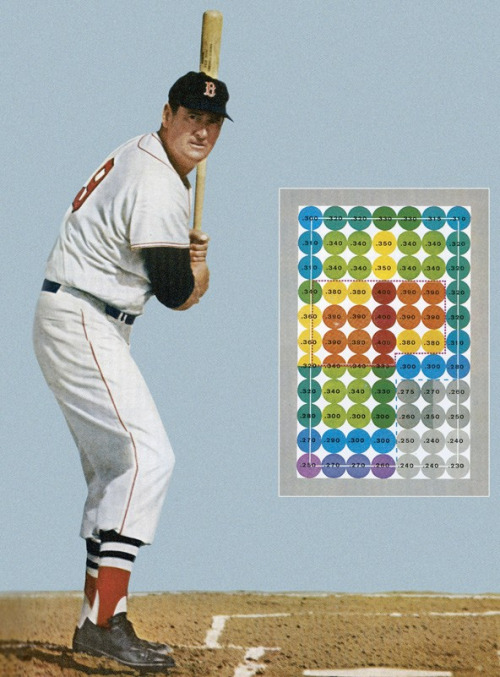
\includegraphics[scale=.35]{Images/Williams.jpg} 
      	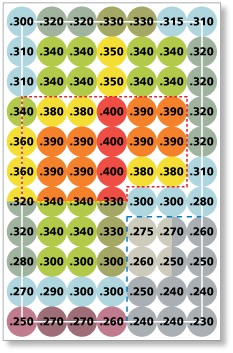
\includegraphics[scale=0.65]{Images/SZ.jpg}
      	\caption{Ted Williams carefully considered which pitch locations he preferred for hitting success. He shows his preferences in this image, where he divided the strike zone into pitch locations with specific probabilities of getting a hit. He labeled the baseballs with personal batting average estimates for pitches in that location \citep{Williams1971}.}
      	\label{fig:Williams}
      	\end{figure} 
In Figure \ref{fig:Williams}, the strike zone is enlarged on the right and contains baseballs labelled with the batting averages Williams estimated he achieved swinging at pitches in that location. Williams based his estimates on experience and intuition, because no such data existed. In fact, it took another 40 years for technology capable of collecting this type of data to make it to MLB\textsuperscript{\textregistered}.

In 2008 MLB collaborated with a company called Sportsvision, Inc to implement a new technology called PITCHf/x\textsuperscript{\textregistered}. PITCHf/x\textsuperscript{\textregistered} collects the data necessary to analyze, visualize, and model Williams's location-based conception of hitting success. In this dissertation we use these data to make three primary ``contributions to knowledge'' \cite{gradguide}.
\begin{enumerate}
\item We develop and introduce variable-resolution (VR) heat maps, a new category of heat map. VR maps work especially well for empirical spatial data with varying abundance through the domain. 
\item We develop and introduce interactive heat map confidence intervals (HMCIs), a new way of presenting HMCIs that makes them easier to understand and interpret.
\item We summarize, use, and assess the computational feasibility of three approaches to fitting Bayesian spatial generalized linear mixed models (SGLMMs) to baseball ``big data.''
\end{enumerate}

Additional contributions of this research include the development and launch of two R packages. One, \verb|varyres|, implements our new VR heat maps; and the second, \verb|mapapp|, implements interactive HMCIs. Both packages, initially, will be hosted on the website GitHub.

In the next section we describe PITCHf/x\textsuperscript{\textregistered} data in detail.

\section{PITCHf/x\textsuperscript{\textregistered} Data} % ============================================
Sportvision, Inc., based in Chicago, provides the technology to collect PITCHf/x\textsuperscript{\textregistered} data. During the 2007 season Sportvision finished installed three high speed stereoscopic cameras in every MLB\textsuperscript{\textregistered} stadium. Each camera takes approximately 20 images of each pitch in flight and determines its path in three dimensions \citep{Fast2010}. Sportsvision licenses PITCHf/x\textsuperscript{\textregistered} data to Major League Baseball Advanced Media (MLBAM\textsuperscript{\textregistered}) \citep{Baumer2010}. 

        \begin{figure}[H]
      	\centering
      	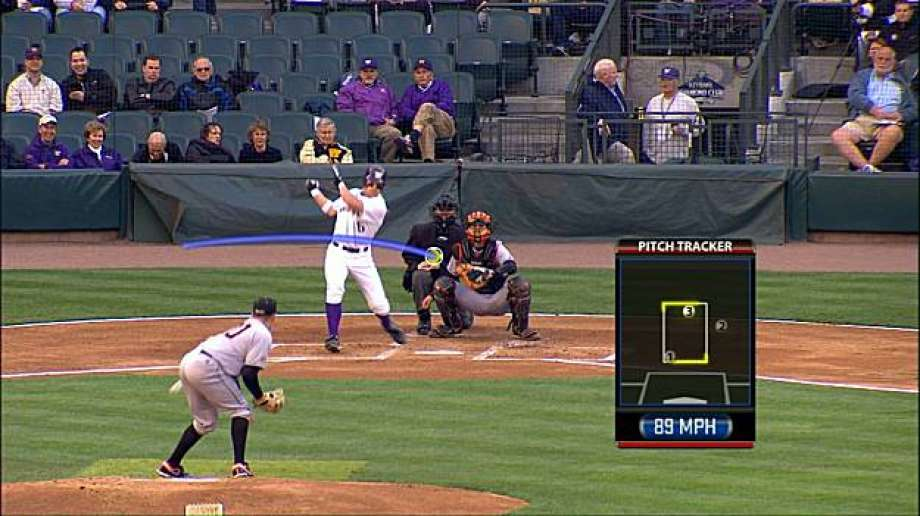
\includegraphics[scale=.4]{Images/PITCHfx.jpg} 
      	\caption{PITCHf/x\textsuperscript{\textregistered} data in your home. Television broadcasts include pitch trajectory and strike zone data, in real time, for the viewer to see.}
      	\label{fig:fx1}
      	\end{figure} 
MLBAM\textsuperscript{\textregistered} makes PITCHf/x\textsuperscript{\textregistered} data publicly available online in XML format, calling it ``Gameday'' data \citep{Sievert2014}. A homepage exists for every game, with links organizing data into XML tables with names such as {\it game, inning, at bat, pitch, team, player}, and {\it umpire} \citep{Sievert2014}. The {\it at bat} table, for example, contains data for 15 variables across 1,711,211 at bats. The format and size---on the order of gigabytes---of the data preclude direct download. Instead, XML scripts automate database ready downloads \citep{Adler2006}. We used a MySQL database, and \verb|dplyr| database management functions in R, to manipulate and store 13 PITCHf/x\textsuperscript{\textregistered} tables \citep{Tahaghoghi2006}, \citep{Wickham2016}. 

As an ``in-memory'' application, R uses a computer's limited RAM to host the R environment data \citep{Smith2013}. As a result, data manipulation on this scale requires ``memory management'' techniques \citep{Wickham2014}.  We applied Split-Apply-Combine operations to tables inside the MySQL database, before importing data frames to R \citep{Wickham2011}.

We collected the variables relevant for this research primarily from the {\it at bat} and {\it pitches} tables. We list these variables, with a short description, below \citep{Fast2007}.
  \begin{description}[leftmargin=1.5cm, style=nextline]
  \item[px] location of the pitch on the horizontal axis when it passes through the strike zone (or the extended plane), recorded in feet from the middle of home plate, from the catcher/umpire point of view.
  \item[pz] location of the pitch on the vertical axis when it passes through the strike zone plane, measured in feet above the ground. A negative value implies the ball bounced before reaching home plate
  \item[des] a short description of the outcome of the pitch, i.e. swing and miss, ground ball for out, ground ball for hit, etc.
  \item[id] a unique id for a pitch within a game.
  \item[ab\_id] a unique id for each at bat.
  \item[pitch\_id] a unique identification number for each pitch.
  \item[pitch\_type] a classification of the type of pitch, out of 18 possible types. For example, four seam fastball, two seam fastball, curveball, knuckle ball, etc.
  \item[stand] handedness of the batter, right or left.
  \item[batter] a unique ID for each hitter.
\end{description}

Professional baseball teams, fans, and the baseball media (TV, radio, print, etc)  continually seek more insightful analysis. The collection and distribution of PITCHf/x\textsuperscript{\textregistered} data comes in response to this demand. In the next section we discuss the relevance of statistical analysis of baseball data, and of our research in particular, to these groups.

\section{Baseball Context and Motivation}

Major League Baseball (MLB\textsuperscript{\textregistered}) teams employ approximately 156 quantitative analysts, at a total cost of approximately \$15 million annually \citep{Lindbergh2016}. Teams strive to gain marginal competitive advantages, so analysis of strike zone data always generates interest. For example, conventional baseball wisdom advises pitchers to ``keep the ball down'' \citep{Stallings2003}; model-based justification for this dictum could help teams intelligently exploit it. Taken further, suppose the model included biomechanical covariates, and biomechanists study the results. MLB\textsuperscript{\textregistered} team scouting departments could use this information to more accurately predict hitting success for amateur players of varying builds and biomechanics, a notoriously difficult but lucrative challenge. 

A second example comes at the individual player level. Some MLB\textsuperscript{\textregistered} hitters, such as Joey Votto, have a keen interest in using the most sophisticated analytics available to understand the keys to their success and failure \citep{Daugherty2015}. Votto, who carries a dog-eared copy of Williams's ``The Science of Hitting'' in his bag, pursues such nuances of his craft. Information obtained from fitting a model to Votto's data alone could indicate otherwise imperceptible strengths and weaknesses to exploit or avoid. 

Regarding media interest, television broadcasts of MLB\textsuperscript{\textregistered} games, such as those on ESPN, TBS, or FOX, regularly integrate PITCHf/x\textsuperscript{\textregistered}-based visuals into the viewing experience \citep{Cross2015}. Figure \ref{fig:fx2} shows a televised baseball graphic made possible by PITCHf/x\textsuperscript{\textregistered}.
        \begin{figure}[H]
      	\centering
      	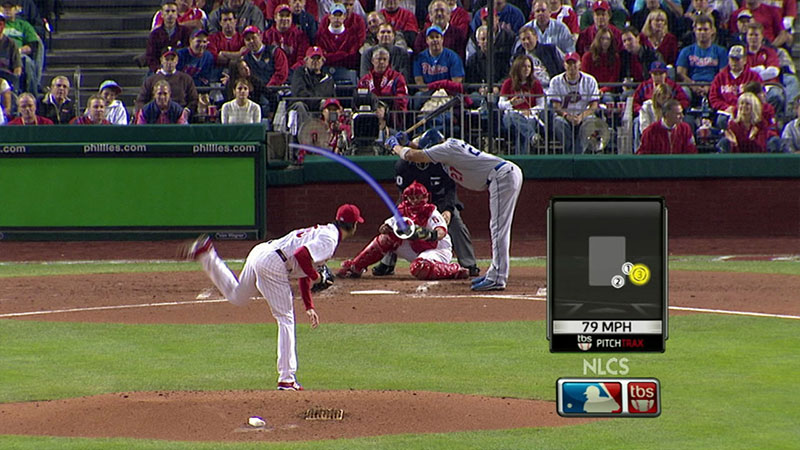
\includegraphics[scale=.4]{Images/PITCHfx2.jpg} 
      	% 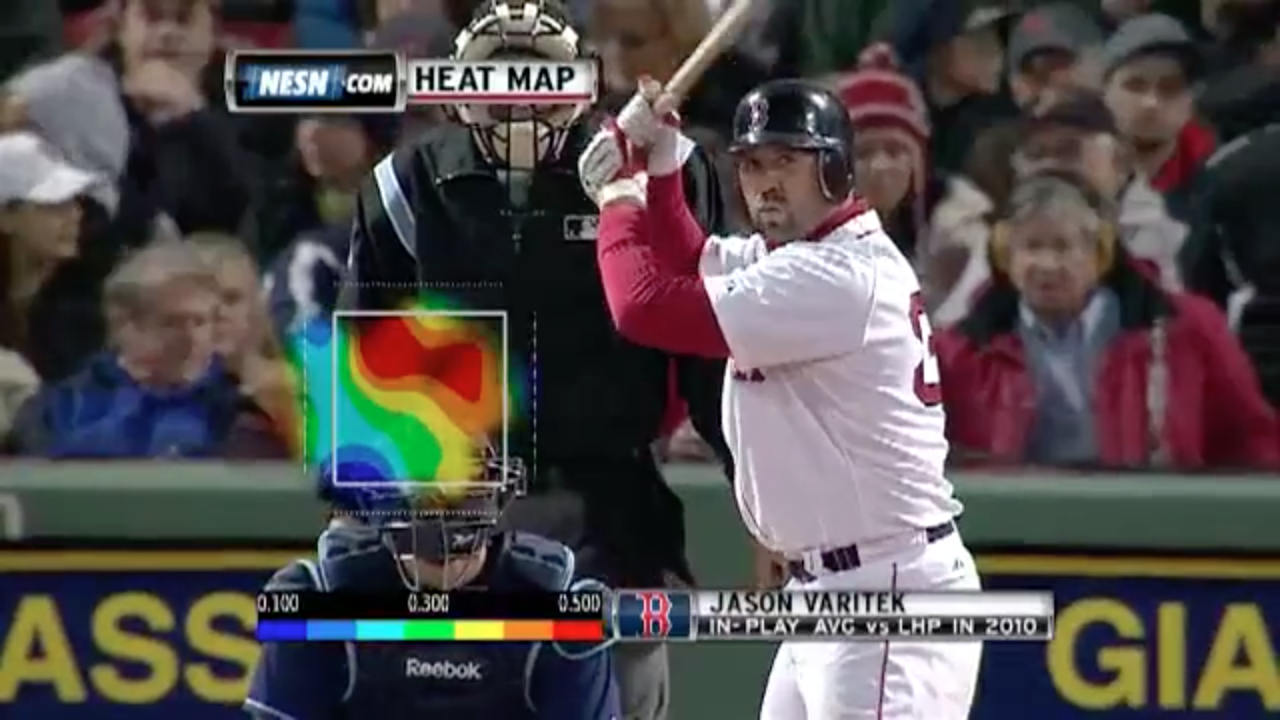
\includegraphics[scale=.25]{Images/Varitek.png} 
      	\caption{PITCHf/x\textsuperscript{\textregistered} data on TV. The graphic shows the pitch's trajectory, and where it passed through the strike zone. The game aired on Turner Broadcast System.} % The lower image includes what appears to be a smoothed empirical heat map on New England Sports Network. We envision an integration of these two visuals.
      	\label{fig:fx2}
      	\end{figure} 
This popular type of PITCHf/x\textsuperscript{\textregistered} display appears frequently on MLB\textsuperscript{\textregistered} broadcasts. The image in Figure \ref{fig:fx3}, from a game on the New England Sports Network, includes a graphic much less common on TV, an actual (perhaps stylized) heat map.
        \begin{figure}[H]
      	\centering
      	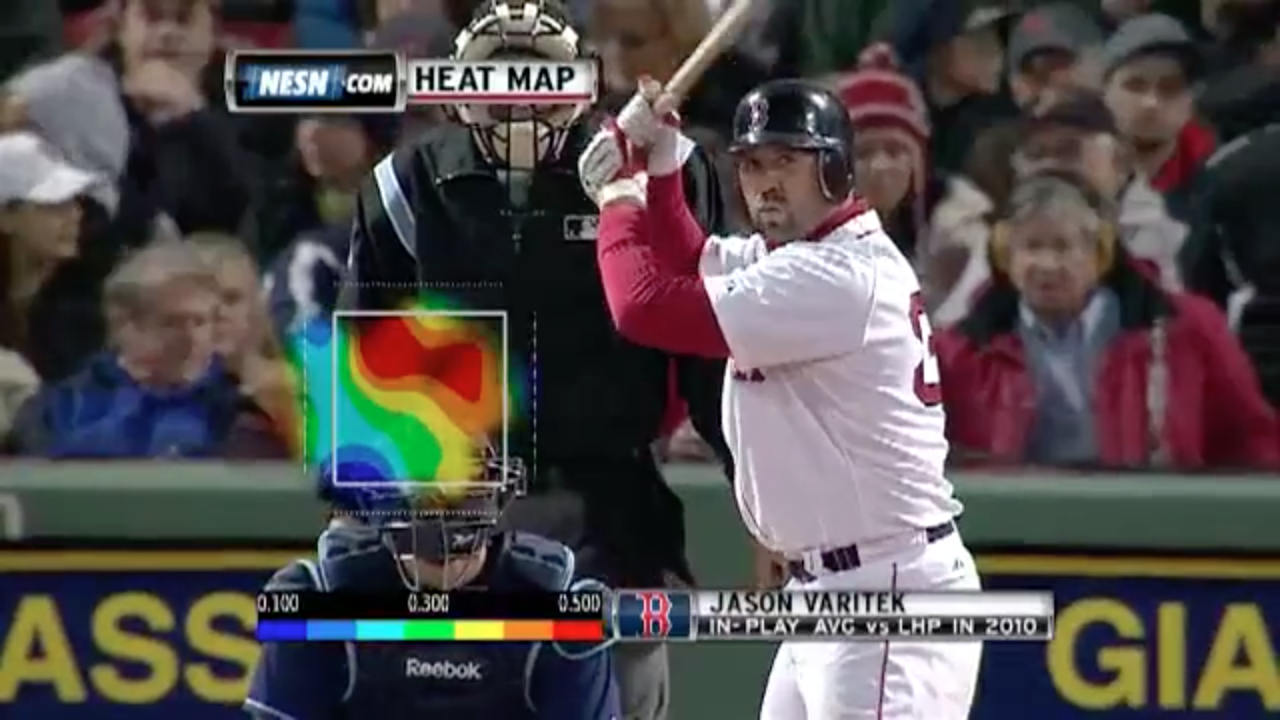
\includegraphics[scale=.25]{Images/Varitek.png} 
      	\caption{PITCHf/x\textsuperscript{\textregistered} data on TV. This image, from a game on the New England Sports Network, includes a smoothed empirical heat map indicating Jason Varitek's spatial success through the strike zone.} 
      	\label{fig:fx3}
      	\end{figure} 
The details of this heat map---the data set and statistical techniques used---are unknown. Nonetheless, improved visuals serve the interests of MLB\textsuperscript{\textregistered} and the networks; ESPN\textsuperscript{\textregistered} and MLB\textsuperscript{\textregistered} recently agreed to an eight year, \$5.6 billion contract \citep{Newman2012}.

As the dollar amounts suggest, the pursuit of insightful analysis rages on. We are in a unique position, with the requisite expertise and data accessibility, to contribute such insightful analysis. In the next section we describe the existing statistical methods and research to provide context for this dissertation.

\section{Statistical Context and Contributions}

% This research includes novel applications of advanced, cutting edge statistical techniques. In addition, as of publication, only one article in a peer reviewed journal focuses on our area of application. This combination---novel application of existing techniques to an unstudied area---constitutes a statistical research contribution. 

From the baseball data, we analyze strike zone data specifically. As of publication, \cite{Cross2015} constitutes the {\it only} statistical analysis of baseball data in a peer reviewed journal. This is a surprise, given the widespread enthusiasm for baseball, until we consider a few obstacles. First, PITCHf/x\textsuperscript{\textregistered} data collection began relatively recently, in 2008. Second, analysis requires proficiency in statistics, programming, and database management. Third, MLB teams, facing the reality of a zero sum game, conduct research in isolation, and rarely share findings. In sum, these factors help explain the paucity of research. However, our efforts rely on ample previous statistical research, and some research outside of statistics.

Our inspiration to model strike zone success owes Ted Williams a debt, for planting the initial seed with ``The Science of Hitting'' \citep{Williams1971}. As for an intersection of baseball and statistical research, \cite{Cross2015} provides the only peer reviewed literature to use as a starting point. The initial heat map in \cite{Cross2015}---on the left in Figure \ref{fig:cross}---illuminated that expressing pitch locations in polar coordinates might help explain spatial variation. 
        \begin{figure}[H]
      	\centering
      	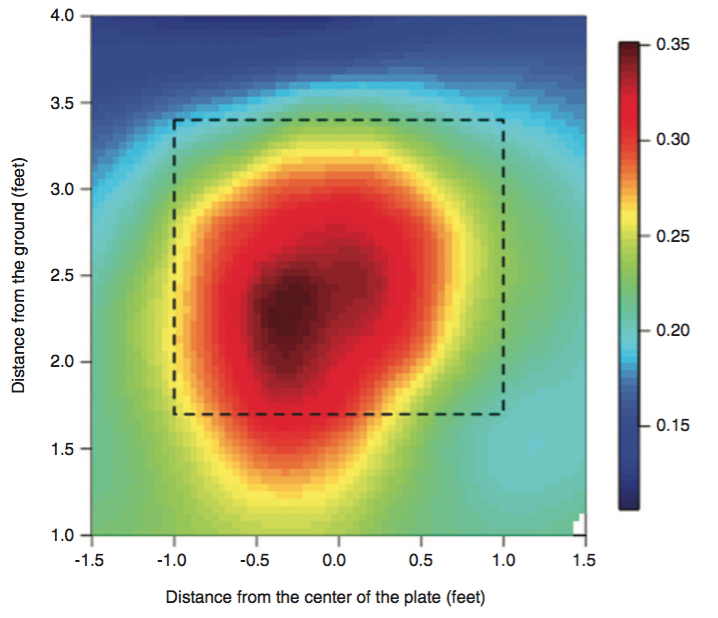
\includegraphics[scale=0.255]{Images/CrossPolar1.jpg} 
      	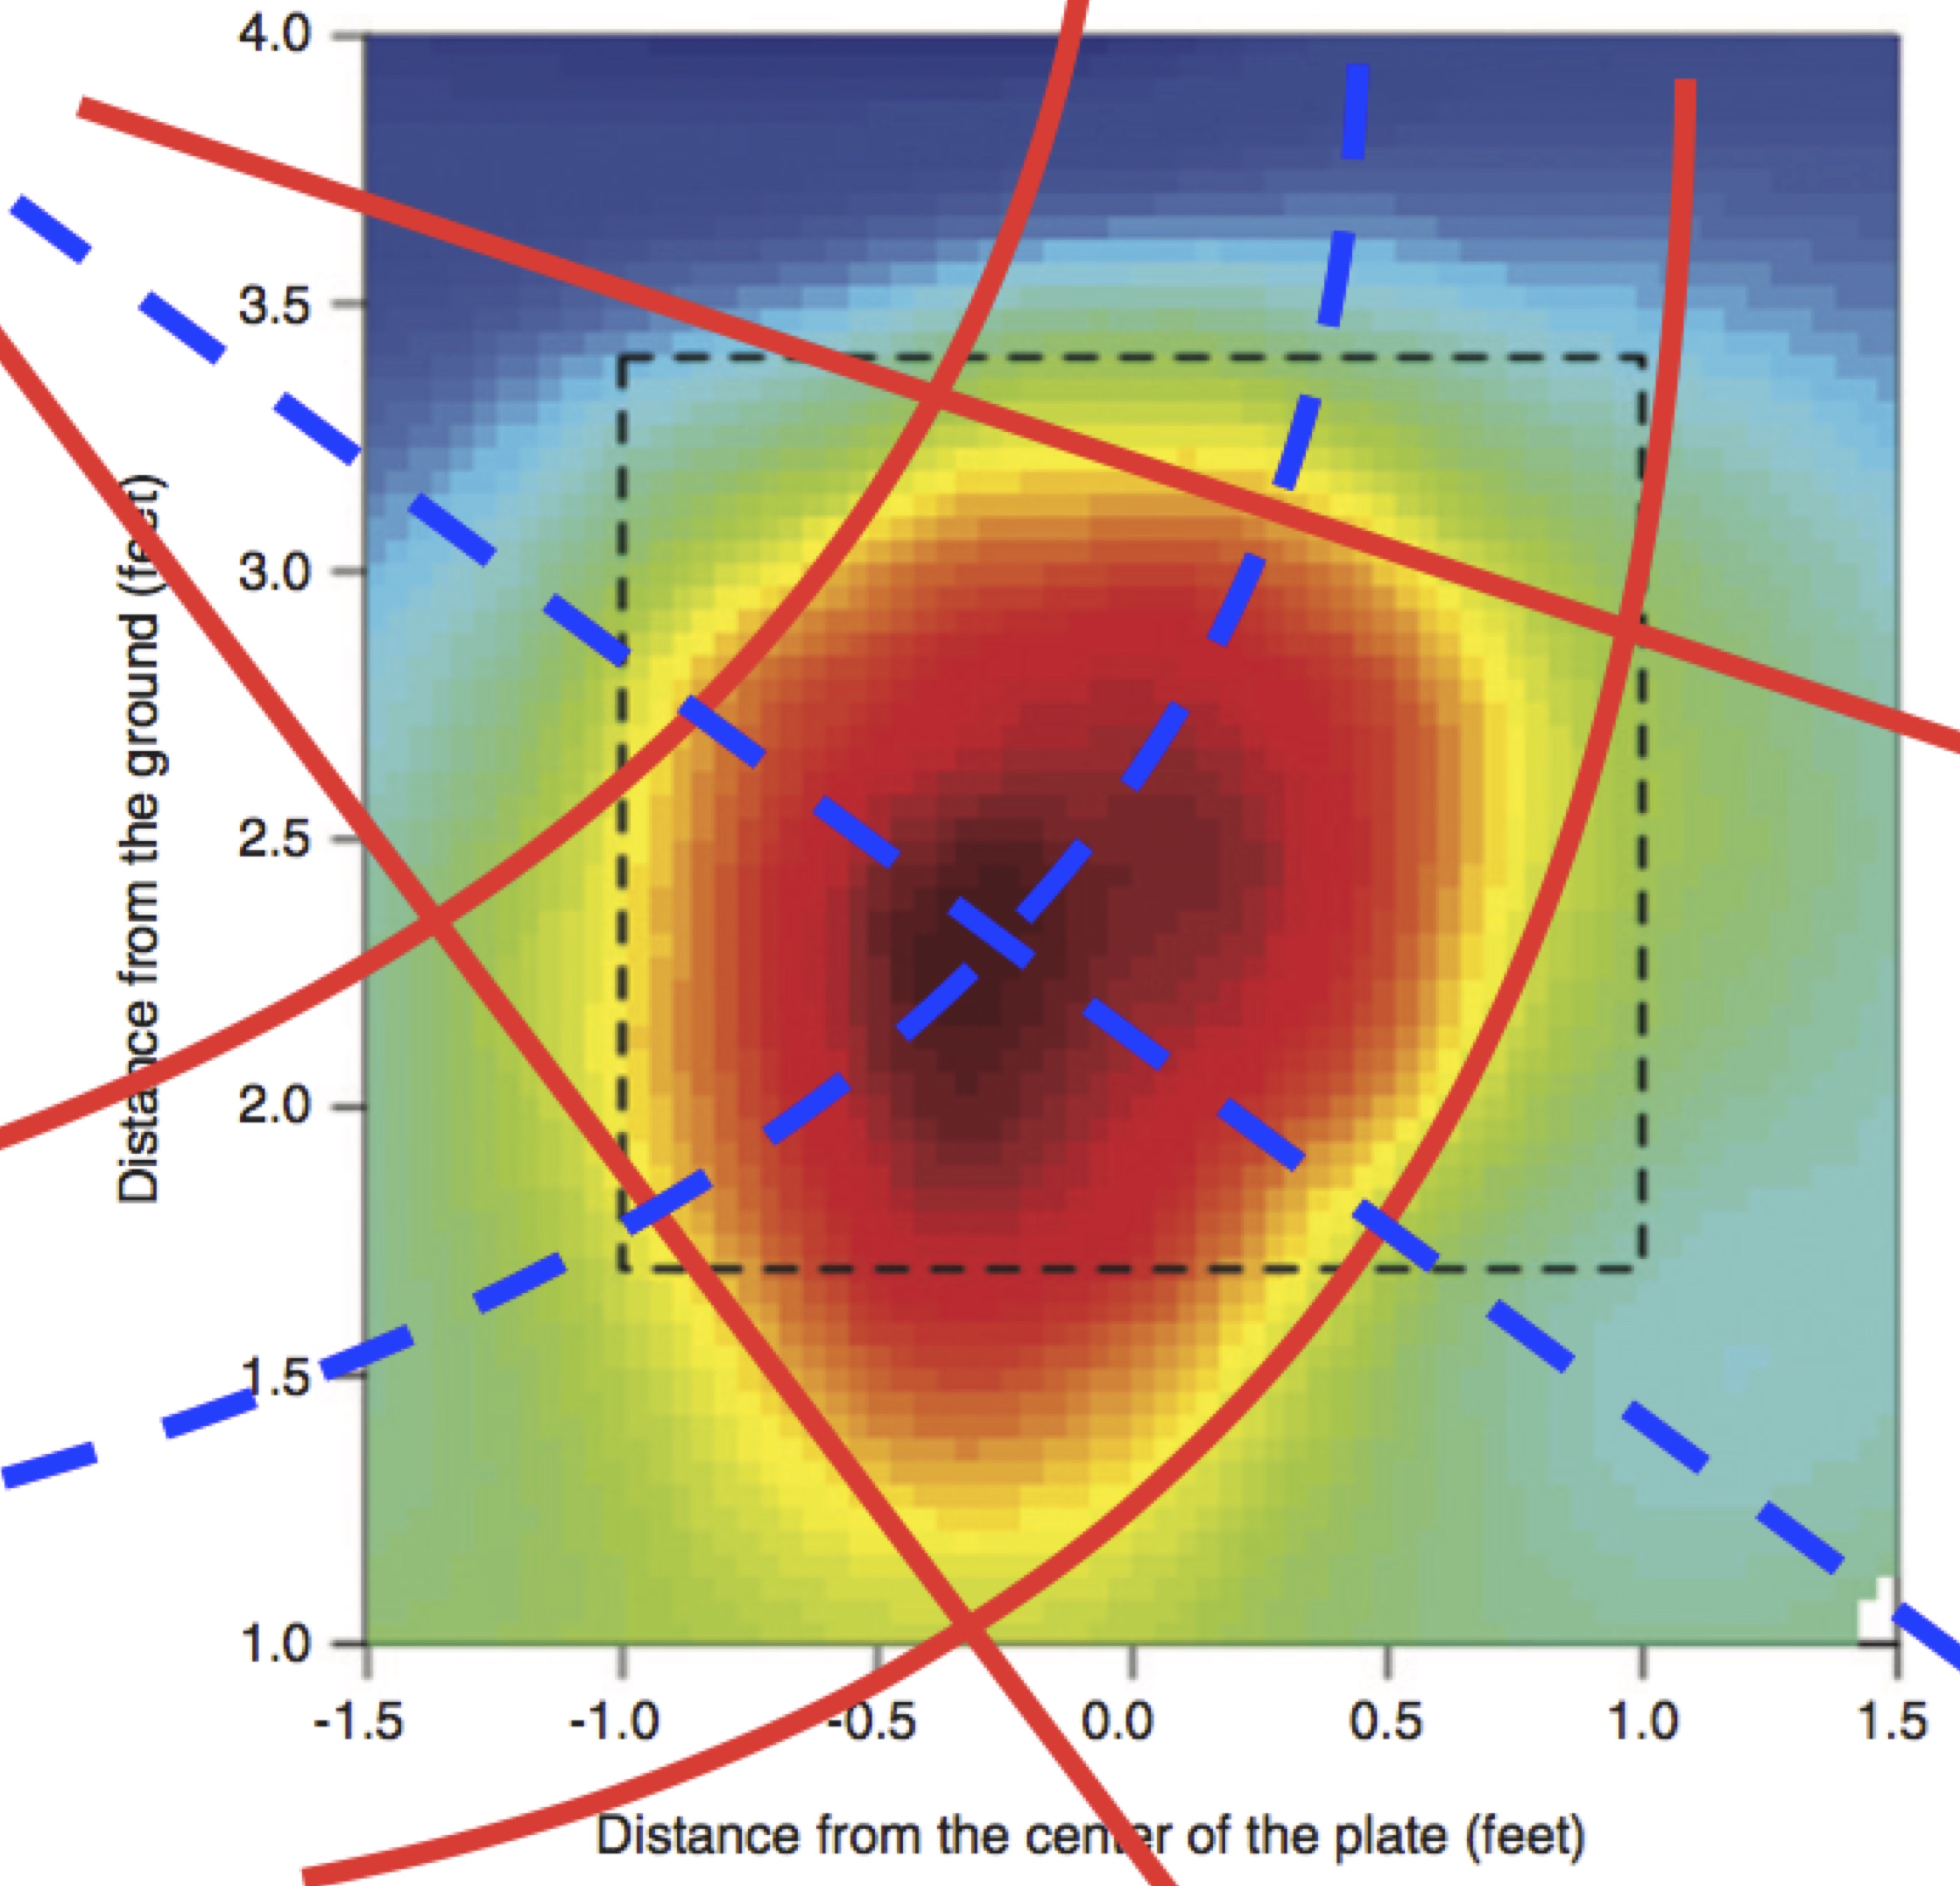
\includegraphics[scale=0.04]{Images/CrossPolar2.jpg} 
      	\caption{\cite{Cross2015} empirical heat map (undisclosed smoothing method) on the left, with lines we added on the right. The general shape of the colored region seems to suggest polar coordinates. We added the radial and angular lines to show how we envisioned polar coordinates helping explain spatial variation.}
      	\label{fig:cross}
      	\end{figure}
The lines we added---shown on the right in Figure \ref{fig:cross}---depict polar coordinates as we envisioned using them. Notice that expressing pitch locations in polar coordinates involves a translated origin. Conducting research into this non-trivial matter, Glenn Fleisig at the American Sports Medical Institute \citep{Fleisig2002} and Brittany Dowling at Motus \citep{Dowling2016} provided feedback and encouragement in personal communications. 

In contrast to \cite{Cross2015} who use kriging to interpolate batting averages\footnote{Calculated as Hits/At Bats.}, we sought a parametric regression model with swing success/failure as the response. \cite{Cross2015} use at bats as observational units, whereas we use swings. Notice that at bats consist of swings, so the at bat as an observational unit is actually just a subset of swings: those that end at bats. This means omitting swinging strikes and foul balls from analysis, which drastically reduces sample sizes. Therefore, we submit that every swing represents a trial, and success/failure to get a hit should be evaluated separately from the count in the at bat at the time of the trial. Accordingly, we define every swing as a Bernoulli trial, with some probability of success. We define success as swings where \verb|des|, short for description, equals \verb|in play, no out|, and failure as swings where \verb|des| equals \verb|Foul|, \verb|Foul (Runner Going)|, \verb|Foul Tip|, \verb|In play out(s)|, \verb|Swinging Strike|, or \verb|Swinging Strike (Blocked)|.

Bernoulli response data suggests a generalized linear model (GLM) with logistic link \citep{Myers2012}. The Hosmer-Lemeshow goodness of fit test validated our polar coordinate based modeling approach \citep{Hosmer2013}. From there, we followed two distinct research paths:
\begin{enumerate}
\item Improving heat map visualizations for our data and analysis, and thus for all spatial data of this nature. This includes adding features to describe uncertainty in estimated probabilities.
\item Addressing the $\mathcal{O}(n^{3})$ increase in computational costs incurred for adding a spatial random effect to our model, known as the ``big N'' problem \citep{Finley2009}. 
\end{enumerate}
Impetus for our two heat map innovations comes from empirical heat maps of PITCHf/x\textsuperscript{\textregistered} data. Hadley Wickham's ``layered grammar of graphics'' in \verb|ggplot2| supplied many of the necessary tools \citep{Wickham2009}, \citep{Wickham2010}; and Doug Nychka's spatial data package \verb|fields| provided critical underlying spatial functions \citep{Nychka}. The second heat map innovation improves the method for presenting heat map confidence intervals. RStudio's ``interactive web application framework'' Shiny provided the new tools necessary for this innovation \citep{Shiny}.

To fit our parametric models, we use Bayesian methodology. This facilitates interpretation of results, and allows for straightforward incorporation of spatial components. Generally speaking Bayesian hierarchical spatial models accommodate a spatial random effect handily \citep{Gelman2014}, \citep{Banerjee2014}, \citep{Oliver2005}. However, we try to fit our model to thousands, and tens of thousands of observations, which leads to {\it big data} challenges. We created a MySQL database, and used \verb|dplyr| for local database management \citep{Wickham2016}, \citep{Tahaghoghi2006}. We used \verb|dplyr| and ``split-apply-combine'' methods for data wrangling \citep{Wickham2016}, \citep{wrangling}. Finally, we took three swings at the ``big N'' problem: computational optimization; dimension reduction; and approximation.

First, we optimized our model-fitting Stan code using available computational techniques \citep{Gelman2015}. Stan developers created the programming language specifically for Bayesian model fitting and analysis; and produced the R interface we used, \verb|rstan| \citep{rstan}. Stan developers Andrew Gelman, Rob Trangucci, and Bob Carpenter offered personal assistance for optimizing code, beyond the techniques explained in the Stan manual \citep{Gelman}, \citep{Trangucci}, \citep{Carpenter}, \citep{STANtheMan}. Broadly speaking, we used techniques based on linear algebra identities, Bayesian model fitting mechanics, and algorithm efficiency.

Second, we employed Predictive Process Models (PPMs), a dimension reduction procedure \citep{Finley2012}. PPMs project process realizations of a model onto a lower dimensioned subspace \citep{Banerjee2008}; this necessarily reduces the computational cost. We implemented this approach with Finley's \verb|spBayes| package \citep{Finley2013}.

Third, we tried an advanced approximation technique. Integrated nested Laplace approximations (INLAs)---a mathematically complex and computationally sophisticated procedure---give speedy estimates for models with a discrete domain \citep{Rue2009}, \citep{Rue2005}. Because our data come from a continuous domain, we use a stochastic partial differential equation (SPDE) to validly translate our domain to qualify for INLA \citep{Lindgren2011}, \citep{Lindstrom2016}. This complex algorithm has strengths and weaknesses; INLA delivers much faster estimates, but they are biased for spatial Bernoulli data \citep{Mondal2017}, \citep{Simpson2012b}, \citep{Rue2009}.

This overview demonstrates how our research relied on the contributions of numerous other statisticians, programmers, scientists, and even a baseball player. Next, we lay out how this dissertation is organized.

\section{Road map}

In Chapter 2 we explore the problem of resolution selection for empirical heat maps, especially those with spatially varying data density. We introduce variable-resolution heat maps, as a method for addressing this problem. In the chapter appendix we provide a vignette for varyres, our VR heat map implementation package. In the first part of Chapter 3 we present a generalized linear model (GLM) for hitter success that includes biomechanical covariates, but no spatial effect. In the second part of Chapter 3, we explain the challenge of heat map confidence intervals, and describe the current best practices. In an effort to improve best practices, we introduce an interactive Shiny application \citep{Shiny}. This chapter appendix includes a vignette for mapapp, our implementation package for interactive HMCIs with Shiny. In Chapter 4 we add a spatial random effect to our GLM, and examine the computational consequences. We implement and compare three methods for fitting our big data spatial GLM.
